%!TEX encoding = UTF-8 Unicode
%!TEX root = ../galgas-book.tex

%--------------------------------------------------------------
\chapter{Tutorial}
%-------------------------------------------------------------

Le but de ce tutorial est de construire en utilisant GALGAS un compilateur d’un langage inspiré de LOGO, qui fournit en sortie un fichier SVG contenant les tracés définis par un programme source LOGO.


Il est rédigé pour être réalisé sur Unix (Linux, Mac OS X).

La génération des fichiers SVG à partir de GALGAS sera faite par un template.

Vous trouverez des informations sur le format SVG sur la page :

\url{http://www.canarlake.org/index.cgi?theme=svg}

\section{Présentation du langage LOGO}

Vous trouverez une description précise du langage à la fin de cette section. Un programme LOGO décrit le déplacement d'une tortue dans un plan. Celle-ci peut effectuer des déplacements en ligne droite et des rotations sur place. La tortue est munie d'un crayon, qui peut être abaissé ou levé. Un déplacement provoque le tracé d'un segment de droite si le crayon est abaissé.

Un programme LOGO est contenu dans un fichier texte, d'extension \texttt{.logo}. Il comprend une liste (éventuellement vide) de sous-programmes, et une liste d'instructions. L'exécution du programme consiste à exécuter cette liste d'instructions, en appelant les sous-programmes qui y figurent. Initialement, la tortue est en (0, 0), sa direction est 0° (horizontale, vers la droite), et le crayon est levé.


\subsection{Quelques exemples}

Voici quelques exemples de programmes LOGO (\refTableau{carreEtoilePentagoneLogo} et \refTableauPage{hexagoneOctogoneLogo}). Le \refTableauPage{logoErreurSemantiques} liste des programmes présentant des erreurs sémantiques : le compilateur qui va être écrit décelera ces erreurs.

\begin{table}[t]
  \centering
  \small

\begin{multicols}{3}

\textbf{Dessin d'un carré}
\begin{lstlisting}
PROGRAM

  ROUTINE trace
  BEGIN
    FORWARD 50 ;
    ROTATE 90 ;
  END

BEGIN
  FORWARD 100 ;
  ROTATE 90 ;
  FORWARD 100 ;
  ROTATE 270 ;
  PEN DOWN ;
  CALL trace ;
  CALL trace ;
  CALL trace ;
  CALL trace ;
END.
\end{lstlisting}

\columnbreak

\textbf{Dessin d'une étoile}
\begin{lstlisting}
PROGRAM

  ROUTINE trace
  BEGIN
    FORWARD 70;
    ROTATE 160;
  END

  ROUTINE trace3
  BEGIN
    CALL trace;
    CALL trace;
    CALL trace;
  END

BEGIN
  FORWARD 200;
  ROTATE 90;
  FORWARD 300;
  ROTATE 270;
  PEN DOWN;
  CALL trace3;
  CALL trace3;
  CALL trace3;
END.
\end{lstlisting}

\columnbreak

\textbf{Dessin d'un pentagone}
\begin{lstlisting}
PROGRAM

  ROUTINE trace
  BEGIN
    FORWARD 70;
    ROTATE 72;
  END

BEGIN
  FORWARD 200;
  ROTATE 90;
  FORWARD 300;
  ROTATE 270;
  PEN DOWN;
  CALL trace;
  CALL trace;
  CALL trace;
  CALL trace;
  CALL trace;
END.
\end{lstlisting}

\end{multicols}

  \caption{Carré, étoile et pentagone en LOGO}
  \labelTableau{carreEtoilePentagoneLogo}
  \ligne
\end{table}


\begin{table}[t]
  \centering
  \small


\begin{multicols}{2}

\textbf{Dessin d'un hexagone}

\begin{lstlisting}
PROGRAM

  ROUTINE trace
  BEGIN
    FORWARD 70 ;
    ROTATE 60 ;
  END

BEGIN
  FORWARD 100 ;
  ROTATE 90;
  FORWARD 100;
  ROTATE 270;
  PEN DOWN;
  CALL trace;
  CALL trace;
  CALL trace;
  CALL trace;
  CALL trace;
  CALL trace;
END.
\end{lstlisting}


\columnbreak

\textbf{Dessin d'un octogone}

\begin{lstlisting}
PROGRAM

  ROUTINE trace
  BEGIN
    FORWARD 70;
    ROTATE 45;
  END

  ROUTINE trace1
  BEGIN
  CALL trace;
  CALL trace;
  END

  ROUTINE trace2
  BEGIN
  CALL trace1;
  CALL trace1;
  END

  ROUTINE trace3
  BEGIN
  CALL trace2;
  CALL trace2;
  END

BEGIN
  FORWARD 100;
  ROTATE 90;
  FORWARD 100;
  ROTATE 270;
  PEN DOWN;
  CALL trace3;
END.
\end{lstlisting}

\end{multicols}

  \caption{Hexagone et octogone en LOGO}
  \labelTableau{hexagoneOctogoneLogo}
  \ligne
\end{table}




\begin{table}[t]
  \centering
  \small

\begin{multicols}{3}

\textbf{Routine récursive}

\begin{lstlisting}
PROGRAM

  ROUTINE routine
  BEGIN
    CALL routine;
  END
  
BEGIN
END.
\end{lstlisting}

\columnbreak

\textbf{Routine indéfinie}

\begin{lstlisting}
PROGRAM

BEGIN
  CALL routine;
END.
\end{lstlisting}

\columnbreak
\textbf{Routine définie plusieurs fois}

\begin{lstlisting}
PROGRAM

  ROUTINE routine
  BEGIN
  END
  
  ROUTINE routine
  BEGIN
  END
  
BEGIN
END.
\end{lstlisting}

\end{multicols}

  \caption{Programmes LOGO contenant des erreurs sémantiques}
  \labelTableau{logoErreurSemantiques}
  \ligne
\end{table}

\subsection{Définition lexicale}

Les identificateurs sont constitués d'une séquence non vide de lettres minuscules ou majuscules. La casse est significative.

Les mots réservés sont les identificateurs suivants : \texttt{PROGRAM}, \texttt{ROUTINE}, \texttt{BEGIN}, \texttt{END}, \texttt{FORWARD}, \texttt{ROTATE}, \texttt{PEN}, \texttt{UP}, \texttt{DOWN} et \texttt{CALL}.

Les constantes littérales entières sont écrites en décimal (une séquence non vide de chiffres décimaux).

Les séparateurs sont l'espace et la fin de ligne.

Les délimiteurs sont le point ('.') et le point virgule (';').

Un commentaire commence par le caractère dièse (\#) et s'étend jusqu'à la fin de la ligne courante.


\subsection {Définition syntaxique}

Un programme LOGO commence le mot réservé \texttt{PROGRAM}, est suivi d'une liste éventuellement vide de définition de routines, du mot réservé \texttt{BEGIN}, d'une liste éventuellement vide d'instructions, et se termine par le mot réservé \texttt{END} suivi d'un point.

Une définition de routine est introduite par le mot réservé \texttt{ROUTINE}, est suivi d'un identificateur, du mot réservé \texttt{BEGIN}, d'une liste éventuellement vide d'instructions, et se termine par le mot réservé \texttt{END}.

Une instruction LOGO est une des séquences suivantes :
\begin{itemize}
  \item le mot réservé \texttt{FORWARD} suivi d'un entier littéral et d'un point virgule ;
  \item le mot réservé \texttt{ROTATE} suivi d'un entier littéral et d'un point virgule ;
  \item le mot réservé \texttt{PEN} suivi du mot réservé \texttt{UP} et d'un point virgule ;
  \item le mot réservé \texttt{PEN} suivi du mot réservé \texttt{DOWN} et d'un point virgule ;
  \item le mot réservé \texttt{CALL} suivi d'un identificateur et d'un point virgule.
\end{itemize}

\subsection{Sémantique statique}

Dans une définition de routine, l'identificateur qui suit le mot réservé \texttt{ROUTINE} est le nom de la routine définie. Dans une instruction \texttt{CALL}, l'identificateur est le nom de la routine appelée.

Contraintes (voir le \refTableau{logoErreurSemantiques} pour des exemples de programmes contenant des erreurs sémantiques) :
\begin{itemize}
  \item le nom d'une routine est unique (on n'a pas le droit de définir plusieurs routines de même nom) ;
  \item une instruction \texttt{CALL} ne peut nommer qu'une routine qui a été définie plus haut dans le texte ;
  \item la routine courante ne peut pas être appelée récursivement.
\end{itemize}

\subsection{Sémantique dynamique}

L'espace de déplacement de la tortue est un plan, muni du repère orthonormé direct habituel. À un instant donné, l'état de la tortue est caractérisé par :
\begin{itemize}
  \item sa position dans le plan ;
  \item sa direction, mesuré en degrés à partir de l'axe horizontal, et dans le sens trigonométrique ;
  \item la position du crayon (levé ou abaissé).
\end{itemize}

Initialement, la position de la tortue est (0, 0), sa direction est 0°, et le crayon est levé.

L'exécution de chaque instruction a l'effet suivant :
\begin{itemize}
  \item l'instruction \texttt{FORWARD} avance la souris dans sa direction d'une longueur égale à la valeur de la constante entière contenue dans l'instruction ; si le crayon est abaissé, un segment de droite délimité par les positions de départ et d'arrivée de la tortue est tracé ;
  \item l'instruction \texttt{ROTATE} fait tourner la tortue dans le sens trigonométrique d'un nombre de degrés égal à la constante contenue dans l'instruction ; aucun tracé n'a lieu, quelque l'état du crayon.
  \item l'instruction \texttt{PEN UP} relève le crayon ;
  \item l'instruction \texttt{PEN DOWN} abaisse le crayon ;
  \item l'instruction \texttt{CALL} exécute le sous-programme nommé dans l'instruction.
\end{itemize}











\section{Installation de GALGAS}

Aller sur la page \url{http://galgas.rts-software.org/download/}

GALGAS est un utilitaire en ligne de commande (sauf sur Mac, pour lequel une application Cocoa est disponible). Vous pouvez :
\begin{itemize}
  \item soit télécharger le binaire correspondant à votre plateforme (pour l'installer, aller à la \refSubsectionPage{installerGalgas}) ;
  \item soit télécharger les sources et les recompiler.
\end{itemize}




\subsection{Téléchargement des sources et compilation}

Télécharger l’archive contenant les sources pour Unix et Mac.

Décompressez cette archive et placer le répertoire obtenu (galgas) dans un répertoire dont le chemin ne contient ni espace ni caractère accentué. C'est important car les chemins utilisés dans les makefile de GALGAS sont relatifs.

Dans la suite de la compilation GALGAS, tous les chemins sont indiqués relativement à ce répertoire, qui sera appelé \texttt{constructionGALGAS}.

Donc, vous devez obtenir à la suite de la décompression le répertoire \texttt{constructionGALGAS/galgas}.

Nous allons maintenant compiler GALGAS. Avec le terminal, sur Linux :
\begin{description}
  \item[ ] \texttt{cd constructionGALGAS/galgas/makefile-unix}
  \item[ ] \texttt{make}
\end{description}

Sur Mac :
\begin{description}
  \item[ ] \texttt{cd constructionGALGAS/galgas/makefile-macosx}
  \item[ ] \texttt{make}
\end{description}

La compilation de GALGAS peut prendre une dizaine de minutes. Deux exécutables sont produits :

\begin{itemize}
  \item \texttt{constructionGALGAS/galgas/makefile-unix/galgas} ;
  \item \texttt{constructionGALGAS/galgas/makefile-unix/galgas-debug}.
\end{itemize}

Les deux exécutables sont fonctionnellement identiques. Le premier est celui que vous utiliserez. Le second est la version debug du premier : il est exécuté avec de nombreuses vérifications internes, ce qui fait qu’il est beaucoup lent. Si le premier plante brutalement, on peut utiliser le second pour déceler si une erreur interne peut être mise en évidence.

La section suivante indique comment installer les binaires obtenus.

\subsectionLabel{Installation}{installerGalgas}


Pour pouvoir appeler les exécutables sans avoir besoin de mentionner un chemin, vous avez plusieurs possibilités :
\begin{itemize}
  \item le copier dans le répertoire \texttt{/bin} :  \texttt{sudo cp galgas /bin/}
  \item le copier dans votre répertoire local \texttt{bin} : \texttt{cp galgas $\sim$/bin/}
\end{itemize}

Attention, le répertoire \texttt{$\sim$/bin} n'existe peut-être pas pour votre compte : il faut alors le créer, et l'ajouter dans la variable \texttt{\$PATH}.

Sur Linux :
\begin{description}
  \item[ ] \texttt{mkdir $\sim$/bin/}
  \item[ ] \texttt{echo \textquotesingle export~PATH=\$PATH:$\sim$/bin\textquotesingle~\textgreater{}\textgreater~/home/user/.bashrc}
\end{description}

Sur Mac :
\begin{description}
  \item[ ] \texttt{mkdir $\sim$/bin/}
  \item[ ] \texttt{echo \textquotesingle export~PATH=\$PATH:$\sim$/bin\textquotesingle~\textgreater{}\textgreater~$\sim$/.bash\_profile}
\end{description}













\section{Création du squelette du compilateur LOGO}

Un projet GALGAS nécessite la mise en place de nombreux fichiers, de créer des makefile pour différentes plateformes, … 

Appeler galgas avec l'option \texttt{-{}-create-project} permet de créer automatique un projet prêt à être utilisé.

Pour tout le tutorial vous devez utiliser un répertoire dont le chemin ne contient ni espace ni caractère accentué. C'est important car les chemins utilisés dans les makefile de GALGAS sont relatifs.

Dans toute la suite de ce tutorial, les chemins sont indiqués relativement à ce répertoire, qui sera appelé \texttt{chezmoi}.

La création :
\begin{description}
  \item[ ] \texttt{cd chezmoi}
  \item[ ] \texttt{galgas -{}-create-project=logo}
\end{description}

Le message affiché par cette opération est :
\begin{description}
  \item[ ] \texttt{*** PERFORM PROJECT CREATION (-{}-create-project=logo option) ***}
  \item[ ] \texttt{*** DONE ***}
\end{description}

L’affichage de \texttt{DONE} indique que la création s’est effectuée avec succès : un répertoire nommé \texttt{logo} a été créé dans le répertoire \texttt{chezmoi}.

\subsection{Visite guidée du répertoire créé}

Dans le répertoire \texttt{chezmoi/logo} :
\begin{itemize}
  \item le fichier \texttt{+logo.galgasProject} est le fichier projet, c’est lui que vous compilerez ;
  \item le répertoire \texttt{galgas-sources} contient les fichiers sources que vous allez compléter tout au long de ce tutorial ; son contenu est indiqué dans le tableau suivant.
\end{itemize}

\begin{table}[t]
  \centering
  \begin{tabular}{ll}
    \textbf{Fichier} & \textbf{Description}\\
    \texttt{logo-lexique.galgas} & Définit l'analyseur lexical\\
    \texttt{logo-semantics.galgas} & Définit les types pour la sémantique\\
    \texttt{logo-syntax.galgas} & Définit les règles de production de la grammaire \\
    \texttt{logo-grammar.galgas} & Définit la grammaire (axiome, classe) \\
    \texttt{logo-program.galgas} & Définit la routine principale \\
    \texttt{logo-cocoa.galgas} & Définit l’interface pour Cocoa : utile uniquement sous Mac \\
    \texttt{logo-options.galgas} & Définit les options de la ligne de commande \\
  \end{tabular}
  \caption{Contenu des sous-répertoires de \texttt{logo} après compilation GALGAS}
  \labelTableau{tableauRepertoireLOGOapresCompGALGAS}
  \ligne
\end{table}






\subsection{Première compilation du projet}

Une compilation s'effectue en deux temps :
\begin{enumerate}
  \item d'abord une compilation GALGAS qui crée ou met à jour des fichiers C++ ;
  \item ensuite une compilation C++.
\end{enumerate}


\subsubsection{Compilation GALGAS}

Vous devez d'abord compiler les sources GALGAS :
\begin{description}
  \item[ ] \texttt{galgas -v chezmoi/logo/+logo.galgasProject}
\end{description}

L'option \texttt{-v} (verbose) provoque l'affichage de messages : observez ceux qui indiquent la création des fichiers C++. Ceux-ci sont rangés dans le répertoire \texttt{chezmoi/logo/build/output} et \texttt{chezmoi/logo/build/libpm}.

Le répertoire \texttt{logo} est complété par de nouveaux répertoires (\refFigure{}{figureRepertoireLOGOapresCompGALGAS} et \refTableau{tableauRepertoireLOGOapresCompGALGAS}).
\begin{figure}[t]
  \centering
  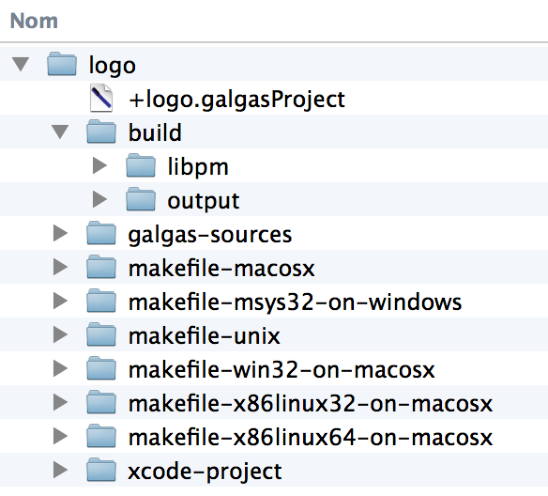
\includegraphics{partie-utilisation/repertoire-logo.pdf}
  \caption{Répertoire \texttt{logo} après compilation GALGAS}
  \labelFigure{figureRepertoireLOGOapresCompGALGAS}
  \ligne
\end{figure}


\begin{table}[t]
  \centering
  \begin{tabular}{ll}
    \textbf{Répertoire} & \textbf{Contenu} \\
    \texttt{makefile-macosx} & Makefile pour compiler sur Mac OS X \\
    \texttt{makefile-msys32-on-windows} & Makefile pour compiler sur Win 32 \\
    \texttt{makefile-unix} & Makefile pour compiler sur Unix \\
    \texttt{makefile-win32-on-macosx} & Makefile pour compiler sur Mac OS X pour Win 32 \\
    \texttt{makefile-x86linux32-on-macosx} & Makefile pour compiler sur Mac OS X pour x86 Linux 32 bits \\
    \texttt{makefile-x86linux64-on-macosx} & Makefile pour compiler sur Mac OS X pour x86 Linux 64 bits \\
    \texttt{xcode-project} & Projet Xcode pour compiler sur Mac OS X
  \end{tabular}
  \caption{Contenu des sous-répertoires de \texttt{logo} après compilation GALGAS}
  \labelTableau{tableauRepertoireLOGOapresCompGALGAS}
  \ligne
\end{table}



\subsubsection{Compilation C++}
Choisissez le répertoire correspondant à votre plateforme (\texttt{makefile-macosx} ou \texttt{makefile-unix}) et lancer le script de compilation \texttt{build.py} (soit via la ligne de commande, soit en double-cliquant).

Par exemple :
\begin{description}
  \item[ ] \texttt{chezmoi/logo/makefile-unix/build.py}
\end{description}

Vous obtenez deux exécutables :
\begin{description}
  \item[ ] \texttt{chezmoi/logo/makefile-unix/logo}
  \item[ ] \texttt{chezmoi/logo/makefile-unix/logo-debug}
\end{description}

Sous Mac, vous pouvez utiliser le projet Xcode engendré, et ainsi créer une application Cocoa nommée \texttt{CocoaLogo}.

Dans tous les cas, comme les analyseurs lexicaux et syntaxiques sont vides après la création, les exécutables ainsi obtenus ne sont pas exploitables.


\section {Analyseur lexical}


Dans cette partie, vous allez écrire l’analyseur lexical du langage LOGO. Pour cela, vous allez modifier le fichier \texttt{chezmoi/logo/galgas-sources/logo-lexique.galgas}.

Remarques préliminaires

1.	en GALGAS, tous les symboles terminaux sont notés par une chaîne de caractères non vide délimitée par deux caractères '\$' ; par exemple : \galgas{$identifier$}, \galgas{$integer$} 

;
2.	en GALGAS, un nom de type est un identificateur précédé du caractère '@' ; par exemple : @string, @uint, @lstring, @luint, … ;
3.	le type @string définit une valeur chaîne de caractères 

;
4.	le type @uint définit une valeur entière non signée sur 32 bits ;
3.	le type @lstring définit une valeur composée d'une chaîne de caractères et d'une information de localisation sur la position de la chaîne dans le texte source 

;
4.	le type @luint définit une valeur composée d'une valeur entière non signée et d'une information de localisation sur la position de la chaîne dans le texte source 

;
5.	ces informations de localisation sont à la base du signalement d'erreur.

\subsection{Analyse lexicale d'un identificateur et d'un mot réservé}

Par défaut, une analyse lexicale des identificateurs et une liste de mots réservés est présente. Tout ce que vous avez à faire est de modifier la liste des mots réservés pour y placer ceux du langage LOGO.

Voici les lignes correspondantes :

\begin{galgascode}
@string tokenString
style keywordsStyle -> "Keywords"
$identifier$ ! tokenString error message "an identifier"

list keyWordList style keywordsStyle error message "the '%K' keyword" {
  "begin",
  "end"
}

rule 'a'->'z' | 'A'->'Z' {
  repeat
    enterCharacterIntoString (!?tokenString !*)
  while 'a'->'z' | 'A'->'Z' | '_' | '0'->'9' :
  end
  send search tokenString in keyWordList default $identifier$
}
\end{galgascode}

Explications :
@string tokenString déclare l’attribut lexical tokenString de type chaîne de caractères ; au début de l’analyse de chaque token, cet attribut est initialisé à la valeur chaîne vide ;
style keywordsStyle -> "Keywords" déclare un style (uniquement utile pour l’application Cocoa engendrée (sur Mac uniquement, vous pouvez ignorer cette ligne) ;
$identifier$ ! tokenString error message "an identifier" déclare le terminal $identifier$ qui sera transmis à l’analyseur syntaxique accompagné de la valeur de tokenString ;  le message d’erreur qui suit est celui qui est utilisé lors d’une erreur syntaxique ;
list keyWordList style keywordsStyle error … déclare une liste de mots réservés associés à un style d’affichage (pour l’application Cocoa sur Mac), un message d’erreur syntaxique ; telle qu’elle est présente, cette définition déclare les deux non terminaux $begin$ et $end$ ;
enfin, rule 'a'->'z' | 'A'->'Z' … effectue l’analyse lexicale des identificateurs en accumulant dans tokenString les caractères rencontrés ; la ligne send search tokenString in keyWordList default $identifier$ recherche un mot réservé et par défaut retourne à l’analyseur syntaxique un identificateur.

Vous n’avez donc qu’à modifier la liste des mots réservés en y plaçant ceux du langage LOGO :
\begin{galgascode}
list keyWordList style keywordsStyle error message "the '%K' keyword" {
  "PROGRAM", "ROUTINE", "BEGIN", "END", "FORWARD",
  "ROTATE",  "CALL",    "PEN",   "UP",  "DOWN"
}
\end{galgascode}

\subsection{Analyse lexicale d'une constante entière}

L’analyse lexicale d’une constante entière 32 bits non signée est présente par défaut, vous n’avez rien à ajouter.

Voici l'écriture correspondante :
\begin{galgascode}
style integerStyle -> "Integer Constants"
@uint uint32value
$integer$ !uint32value style integerStyle error message "a 32-bit unsigned decimal number"

message decimalNumberTooLarge : "decimal number too large"
message internalError : "internal error"

rule '0'->'9' {
  enterCharacterIntoString (!?tokenString !*)
  repeat
  while '0'->'9' :
    enterCharacterIntoString (!?tokenString !*)
  while '_' :
  end
  convertDecimalStringIntoUInt (!tokenString !?uint32value error decimalNumberTooLarge, internalError)
  send $integer$
}
\end{galgascode}


Explications :
style integerStyle -> "Integer Constants" déclare un style (uniquement utile pour l’application Cocoa engendrée (sur Mac uniquement, vous pouvez ignorer cette ligne) ;
@uint uint32value déclare l’attribut lexical uint32value de type entier 32 bits non signé ; au début de l’analyse de chaque token, cet attribut est initialisé à la valeur zéro ;
$integer$ !uint32value style integerStyle … déclare le terminal $integer$ qui sera transmis à l’analyseur syntaxique accompagné de la valeur de uint32value ;  le message d’erreur qui suit est celui qui est utilisé lors d’une erreur syntaxique ;
message decimalNumberTooLarge : "decimal number too large" déclare un message d’erreur ;
enfin rule '0'->'9' … définit l’analyse lexicale d’une contante entière non signé ; les caractères qui la composent sont accumulés dans tokenString, et la routine convertDecimalStringIntoUInt effectue la conversion de cette chaîne en entier ; pour finir, send $integer$ envoie le terminal vers l’analyseur syntaxique.

\subsection{Analyse des délimiteurs}
Par défaut, un certain nombre de délimiteurs sont définis :

\begin{galgascode}
style delimitersStyle -> "Delimiters"
list delimitorsList style delimitersStyle error message "the '%K' delimitor" {
  ":",    ",",    ";",   "!",  "{",  "}", "->", "@", "*", "-"
}

rule list delimitorsList
\end{galgascode}

La règle précédente déclare les terminaux \galgas{\$:\$}, \galgas{\$,\$}… Les messages d'erreur syntaxique sont définis en remplaçant la séquence \galgas{\%K} par l’épellation du délimiteur.

L'analyse des délimiteurs est définit par la règle rule list delimitorsList.

Travail à faire : remplacer la liste des délimiteurs par celle du langage LOGO.

\subsection{Analyse des chaînes de caractères}
Une analyse des chaînes de caractères est disponible par défaut. Comme le langage LOGO n’utilise pas de chaînes de caractères, vous pouvez supprimer les définitions suivantes :

\begin{galgascode}
style stringStyle -> "String Constants"
$literal_string$ ! tokenString style stringStyle %nonAtomicSelection error message "a character string constant \"...\""

message incorrectStringEnd : "string does not end with '\"'"

rule '"' {
  repeat
  while ' ' | '!' | '#'-> '\uFFFD' :
    enterCharacterIntoString (!?tokenString !*)
  end
  select
  case '"' :
    send $literal_string$
  default
    error incorrectStringEnd
  end
}
\end{galgascode}

\subsection{Analyse des séparateurs}
C'est une règle très simple, qui accepte tout caractère de code ASCII compris entre 0x01 et 0x20 (l'espace). Comme il n'y a pas d'instruction send dans la règle lexicale, l'occurrence d'un séparateur est complètement ignorée par l'analyseur syntaxique.
rule '\u0001' -> ' ' :
end rule ;
La séquence d'échappement \u permet d'écrire directement des points de code Unicode sous la forme de quatre chiffres hexadécimaux.

\subsection{Analyse des commentaires}
C'est un peu plus compliqué, il faut repérer la fin de la ligne courante. Or, celle-ci peut être un seul caractère LF (fichier Unix), un seul caractère CR (fichier Mac Classic), une séquence CRLF (fichier Windows). D'autre part, une ligne de commentaire peut être la dernière ligne du fichier : notez que GALGAS rajoute automatiquement le caractère \galgas{'\\0'} à la fin de la chaîne source. L'analyse d'un commentaire consiste donc, une fois le caractère initial \galgas{'\#'} repéré, à accepter silencieusement tous les caractères possibles, sauf '\\u000A' (LF), '\\u000D' (CR), '\\0'. L’écriture drop \galgas{$comment$} signifie que le terminal $comment$ n’est pas transmis à l’analyseur syntaxique.

\begin{galgascode}
style commentStyle -> "Comments"
$comment$ style commentStyle %nonAtomicSelection error message "a comment"
rule '#' {
  repeat
  while '\u0001'->'\u0009' | '\u000B' | '\u000C' | '\u000E'->'\uFFFD':
  end
  drop $comment$
}
\end{galgascode}

Remarquez que pour un fichier Windows, le caractère CR marque la fin du commentaire, et que le caractère LF qui suit est silencieusement absorbé comme délimiteur.

Travail à faire
écrivez l'analyseur lexical du langage LOGO. Après compilations GALGAS et C++, les exécutables logo et logo-debug obtenus sont partiellement opérationnels (pas encore d’analyseur syntaxique) : avec l'option --mode=lexical-only, vous pouvez faire afficher la liste des symboles terminaux produite par l'analyse lexicale du fichier source passé en argument.

Note : l'option --help permet d'afficher la liste des options de l'exécutable. 

\section{Analyseur syntaxique}

Deux fichiers sont concernés :
\begin{itemize}
  \item chezmoi/logo/galgas-sources/logo-syntax.galgas, et
  \item chezmoi/logo/galgas-sources/logo-grammar.galgas.
\end{itemize}

Le fichier logo-syntax.galgas contient une liste de règles de production. Le fichier logo-grammar.galgas définit une grammaire.

Le fichier logo-grammar.galgas
Ce fichier a la composition suivante :

\begin{galgascode}
grammar logo_grammar "LL1" {
  syntax logo_syntax
  <start_symbol>
}
\end{galgascode}

Explications :
LL1 est la classe de la grammaire ;
\galgas{syntax logo_syntax} : les règles de productions sont dans le composant syntaxique logo\_syntax, situé dans le fichier logo-syntax.galgas ; 
\galgas{<start_symbol>} : l'axiome de la grammaire.

A priori, vous n'avez pas besoin de modifier le fichier logo-grammar.galgas au cours du TP. Vous pouvez cependant modifier l'analyse effectuée en suivant les indications du tableau suivant :
Chaîne	Commentaire
"LL1"	Effectue une analyse LL (1) de la grammaire ; échoue si la grammaire n'est pas LL (1).
"SLR"	Effectue une analyse SLR de la grammaire ; échoue si la grammaire n'est pas SLR.
"LR1"	Effectue une analyse LR (1) de la grammaire ; échoue si la grammaire n'est pas LR (1).
""	Effectue une analyse LL (1) de la grammaire ; en cas d'échec, effectue une analyse SLR ; en cas de nouvel échec, effectue une analyse LR (1). 
Rappel :
toute grammaire LL(1) est SLR ;
toute grammaire SLR est LR(1).

Le fichier \galgas{logo_syntax.galgas}
Par défaut, seul le non terminal \galgas{<start_symbol>} est déclaré, et une règle de production vide est écrite.

C'est à vous d'écrire les règles de production qui définissent le langage LOGO (voir sa définition syntaxique en annexe 2).

Voici les indications qui vous permettront d'écrire ces règles :
\begin{itemize}
  \item vous pouvez déclarer autant de non terminaux que vous voulez ;
  \item la forme d'une règle de production est :
				\galgas{rule <mon_non_terminal> { partie droite }}
  \item la partie droite est une séquence éventuellement vide de :
	terminaux ;
	non-terminaux ;
	d'instructions de répétition syntaxique (voir annexe 6) ;
	d'instruction de sélection syntaxique (voir annexe 6).
  \item les règles de production peuvent apparaître dans un ordre quelquonque.
\end{itemize}

Pour vous aider, voici une écriture possible de la dérivation de l'axiome :

\begin{galgascode}
rule <start_symbol> {
#-- Definition des routines
  $PROGRAM$
  repeat
  while
    <routine_definition>
  end
#--- Programme principal
  $BEGIN$
  <instruction_list> 
  $END$
  $.$
}
\end{galgascode}

Et la règle de production \galgas{<routine_definition>} :

\begin{galgascode}
rule <routine_definition> {
  $ROUTINE$
  $identifier$ ?*
  $BEGIN$
  <instruction_list>
  $END$
}
\end{galgascode}

Noter l’écriture \galgas{$identifier$ ?*} : en effet, quand l’analyseur lexical envoie vers l’analyseur syntaxique le token $identifier$, celui-ci est accompagné d’une chaîne de caractère. On indique que la valeur de celle-ci n’est pas utilisée (pour le moment) par l’écriture ?*.

Il en est de même pour le token $integer$ qui est accompagné d’une valeur entière.

Si des erreurs d'analyse de la grammaire surviennent, vous pouvez utiliser l'option --output-html-grammar dans la ligne de commande : celle-ci provoque la génération du fichier :
	\galgas{chezmoi/logo/build/helpers/logo_grammar.html} 
qui contient tous les détails de l'analyse de la grammaire.

À l'issue de ce travail, l'exécutable obtenu doit analyser correctement les programmes LOGO contenus sur le serveur pédagogique.

Vous pouvez utiliser l'option --mode=syntax-only pour afficher la trace de l'analyse syntaxique.

V - Sémantique statique

Le but de cette étape est d'enrichir les fichiers GALGAS de façon à vérifier la sémantique statique du langage LOGO (voir annexe 3).

Préliminaire : obtenir la valeur des identificateurs

Dans l’analyseur syntaxique, pour chaque occurrence du token $identifier$, nous avons écrit $identifier$ ?* pour signifier que la valeur de la chaîne de caractères n’était pas utilisée.

À partir de maintenant, nous avons besoin de cette valeur. Celle-ci est récupérée en écrivant :
$identifier$ ?let @lstring unNom
Cette écriture déclare une constante locale, nommée unNom, de type @lstring.

Notez que le type mentionné est @lstring, alors que dans l’analyseur lexicale une valeur de type @string est associée au terminal $identifier$. Le type @lstring est une structure composée d’une valeur de type @string et d’une valeur de type @location. Cette dernière désigne un point dans le texte source analysé. Lors de la transmission des informations de l’analyseur lexical vers l’analyseur syntaxique, la valeur de type @string est associée à la position de l’identificateur dans le texte source. Ceci permet de construire facilement des messages d’erreur qui désigne l’endroit dans le texte source où l’erreur est apparue.

Pour le moment, on ne modifie pas les terminaux $integer$ :

Faire les modifications et recompiler. Comme les valeurs récupérées ne sont pas utilisées et perdues, vous obtenez un warning pour chaque constante.

Vous pouvez afficher la valeur obtenue en ajoutant une instruction log à chacune des séquences précédentes :
$identifier$ ?let @lstring unNom
log unNom
L'instruction log affiche la valeur d'une variable ou d’une constante. Elle est utilisable sur tous les types GALGAS.

Principes d'écriture de la sémantique
Le cadre général est celui des grammaires attribuées. Ceci revient à doter de paramètres formels les non terminaux de la partie gauche d'une règle, de la même façon que la définition d'une fonction C peut présenter des paramètres formels. En conséquence, un non-terminal apparaissant en partie droite d'une règle de production doit présenter des arguments effectifs, de la même façon qu'un appel de fonction doit citer des arguments effectifs en accord avec la déclaration du prototype de la fonction. Dès lors, vous pouvez établir les correspondances suivantes :
En C	En GALGAS
Le prototype d'une fonction cite la liste des arguments formels.	La déclaration d'un non-terminal cite la liste des attributs (au sens des grammaires attribuées).
L'en tête de l'implémentation d'une fonction cite la liste des arguments formels.	Le non terminal de gauche d'une règle de production cite la liste des attributs (au sens des grammaires attribuées).
L'appel d'une fonction cite des paramètres effectifs.	Un non terminal apparaissant dans la partie droite d'une règle de production cite une liste des attributs (au sens des grammaires attribuées).

En GALGAS, nous utilisons plutôt le vocabulaire des langages de programmation : argument formel, paramètre effectif.

Arguments formels en GALGAS
Un argument formel cite :
\begin{itemize}
  \item un délimiteur qui précise le sens de transmission de l'argument formel ;
  \item son type (par exemple @lstring, @luint, …) ;
  \item son nom.
\end{itemize}


Le sens de transmission d'un argument formel est défini dans le tableau suivant 

:
Délimiteur	Sens de transmission
?	Entrée
?let	Entrée constant
!	Sortie
?!	Entrée/sortie

Paramètres effectifs en GALGAS
Un paramètre effectif cite :
\begin{itemize}
  \item un délimiteur qui précise le sens de transmission du paramètre effectif ;
  \item une variable locale ou un argument formel de la règle de production.
\end{itemize}

Le sens de transmission d'un paramètre effectif est défini dans le tableau suivant 

:
Délimiteur	Sens de transmission	Argument formel correspondant
?	Entrée	! (argument formel en sortie)
!	Sortie	? (argument formel en entrée) ou
?let (argument formel en entrée constant)
!?	Sortie/entrée	?! (argument formel en entrée/sortie)

Les types en GALGAS
Il existe plusieurs sortes de types :
\begin{itemize}
  \item les types prédéfinis par le langage, comme @lstring, @luint, … ;
  \item les types définis par l'utilisateur, qui peuvent être :
	des types table ;
	des types liste ;
	des types classe.
\end{itemize}

écriture de la sémantique statique
Pour décrire la sémantique statique (voir annexe 3), le plus simple est de créer un type table de symboles, dont une instance contiendra tous les noms de routines d'un programme LOGO.

Ajout du type de table des routines
éditez le fichier chezmoi/logo/galgas-sources/logo-semantics.galgas et ajouter la définition suivante :

\begin{galgascode}
map @routineMap {
  insert insertKey error message "the '%K' routine has been already declared"
  search searchKey error message "the '%K' routine is not declared"
}
\end{galgascode}

Ceci déclare le type @routineMap, avec une méthode d'insertion insertKey accompagnée de son message d'erreur, et une méthode de recherche searchKey accompagnée de son message d'erreur. Implicitement, la clé de la table est du type @lstring.

Cette définition sera complétée dans l'étape suivante afin de prendre en compte les instructions des routines (on n'en a pas besoin pour le moment).

À cet instant, vous pouvez recompiler le fichier logo-semantics.galgas.

Instructions sur les objets de type table
Voici quatre instructions relatives aux tables dont vous allez avoir besoin :
\begin{itemize}
  \item la déclaration d'un objet de type table ;
  \item l'initialisation d'un objet de type table ;
  \item l'instruction d'insertion dans une table ;
  \item l'instruction de recherche dans une table.
\end{itemize}

La déclaration d'un objet de type table se fait simplement en nommant le type puis l'objet ; par exemple :
	@routineMap maTable

L'initialisation d'un objet de type table s'effectue en appelant le constructeur emptyMap, qui crée une table vide :
	maTable = {}

Les deux écritures précédentes peuvent condensées en une seule par :
	@routineMap maTable = {}

L'instruction d'insertion dans une table est :
	[!?maTable insertKey !clef]
où insertKey est le nom d'une méthode d'insertion déclarée dans le type table ; clef doit être une variable de type @lstring valuée. Si il existe déjà une entrée de même nom, le message d'erreur associé à la méthode d'insertion est affiché.

L'instruction de recherche dans une table est :
	[maTable searchKey !clef]
où searchKey est le nom d'une méthode de recherche déclarée dans le type table ; clef doit être une variable de type @lstring valuée. Si il n'existe pas d'entrée de même nom, le message d'erreur associé à la méthode de recherche est affiché.

Ajout de la sémantique dans les règles de productions
éditer le fichier chezmoi/logo/galgas-sources/logo-syntax.galgas et modifiez la dérivation de l'axiome :

\begin{galgascode}
rule <start_symbol> {
  $PROGRAM$
  @routineMap tableRoutines = {}
  repeat
  while 
    <routine_definition> !?tableRoutines
  end
  $BEGIN$
  <instruction_list>
  $END$
  $.$
}
\end{galgascode}

L'appel du non terminal\galgas{<routine_definition>} impose que son en-tête doit être modifiée en conséquence :
\begin{galgascode}
rule <routine_definition> ?!@routineMap ioTableRoutines {
  ...
}
\end{galgascode}

Travail à faire
Maintenant, à vous de compléter les règles de façon à prendre en compte toutes les contraintes édictées en annexe 3.

Vérifiez que votre analyseur détecte correctement les erreurs. Pour cela, vous pouvez utiliser les exemples suivants disponibles sur le serveur pédagogique :
\begin{itemize}
  \item erreur\_appel\_recursif.logo ;
  \item erreur\_routine\_definie\_plusieurs fois.logo ;
  \item erreur\_routine\_indefinie.logo.
\end{itemize}

\section{Sémantique dynamique}

Dans la sémantique dynamique (annexe 4), nous allons prendre en compte la signification de l'exécution d'une instruction. En préliminaire, nous allons compléter l'analyseur lexical pour qu'il envoie la valeur d'une constante entière.

Préliminaire : les constantes entières

Modifier maintenant l’analyse syntaxique des constantes entières, à l’image de ce qui a été fait pour les identificateurs :
\begin{galgascode}
$integer$ ?let @luint unNom
\end{galgascode}

Le type @luint est une structure composée d’une valeur de type @uint et d’une valeur de type @location.

Mise à plat de la liste des instructions
Le but ultime est d'obtenir la liste des instructions du programme principal. Mais quelles sont les instructions qui devront apparaître dans cette liste ? A priori, toutes les instructions décrites dans l'annexe 4. En fait, vous pouvez vous passer de l'instruction CALL en insérant dans la liste des instructions non pas cette instruction, mais la liste des instructions de la routine correspondante. Il faut procéder de même lors de construction de la liste de chaque routine.

Hiérarchie des classes des instructions
Une solution classique pour ce type de situation est de définir une classe abstraite @instruction, et des classes concrètes @penUp, @penDown, @rotate et @forward qui héritent de cette classe abstraite :écriture des classes dans le composant sémantique éditez le fichier chezmoi/logo/galgas-sources/logo-semantics.galgas et insérer le texte suivant, avant la déclaration du type table :

\begin{galgascode}
abstract class @instruction {
}
class @penUp : @instruction {
}
class @penDown : @instruction {
}
class @forward : @instruction {

@luint mLength
}
class @rotate : @instruction {

@luint mAngle
}
\end{galgascode}


Les trois premières classes n'ont pas d'attribut, et les deux dernières un attribut de type @luint.

Instructions sur les objets de type class
Vous avez besoin de deux instructions relatives aux classes :
\begin{itemize}
  \item la déclaration d'une variable de type classe ;
  \item l'instanciation d'un objet de type class.
\end{itemize}

La déclaration d'un référence de type classe se fait simplement en nommant le type puis l'objet ; par exemple :
	@instruction instruction

L'instanciation d'un objet de type classe s'effectue en appelant le constructeur new d'une classe concrète avec les paramètres effectifs correspondants aux attributs de la classe, précédés des paramètres effectifs correspondants aux attributs des classes héritées :
	instruction = @rotate.new {!valeurAngle}

Les deux instructions peuvent réduites en :
	@instruction instruction = @rotate.new {!valeurAngle}

Travail à faire
Compléter les règles de productions pour chaque instruction (sauf l'instruction CALL).

Le type liste d'instructions
Pour construire la liste des instructions, il faut définir un nouveau type dont les valeurs sont des listes.

éditez le fichier chezmoi/logo/galgas-sources/logo-semantics.galgas et insérer le texte suivant, après les déclarations de classes et avant la déclaration du type table :

\begin{galgascode}
list @instructionList {
  @instruction mInstruction
}
\end{galgascode}

Ceci déclare le type de liste @instructionList, dont chaque élément contient un objet instance d'une classe héritière de @instruction.

Instructions sur les objets de type liste
Voici trois instructions relatives aux listes dont vous allez avoir besoin :
\begin{itemize}
  \item la déclaration d'un objet de type liste ;
  \item l'initialisation d'un objet de type liste ;
  \item l'instruction d'ajout d'une valeur à une liste.
\end{itemize}

La déclaration d'un objet de type liste se fait simplement en nommant le type puis l'objet 

; par exemple :
	@instructionList maListe

L'initialisation d'un objet de type liste s'effectue en appelant le constructeur emptyList, qui crée une liste vide :
	maListe = {}

Les deux écritures précédentes peuvent condensées en une seule par :
	@instructionList maListe := {}

L'instruction d'ajout d'une valeur dans une liste est :
	maListe += !instruction
L'ajout s'effectue toujours à la fin de la liste.

Travail à faire
Compléter les règles de productions construire la liste des instructions d'une routine et la liste des instructions du programme principal (les instructions CALL sont toujours ignorées).

Modification du type table @routineMap
Pour prendre en compte l’instruction CALL, nous allons procéder comme suit : d’abord, la définition du type table @routineMap va être modifier de façon à associer à chaque routine la liste mise à plat des instructions. Ensuite, nous prendrons en compte l’instruction CALL en extrayant de la table des routine la liste des instructions de la routine appelée, et en l’insérant à la fin de la liste courante des instructions.

Modification du type table @routineMap
Il faut maintenant modifier la définition du type table @routineMap de façon qu'à chaque nom de routine soit associée sa liste d'instructions :

\begin{galgascode}
map @routineMap {
  @instructionList mInstructionList
  insert insertKey  error message "the '%K' routine has been already declared"
  search searchKey error message "the '%K' routine is not declared
}
\end{galgascode}

Recompiler les sources GALGAS, et examiner les erreurs produites. Corrigez les en vous aidant des explications suivantes :
\begin{itemize}
  \item l'instruction d'insertion doit maintenant nommer un argument effectif en sortie supplémentaire, de type @instructionList :
[!?maTable insertKey !clef !maListe] ;
  \item l'instruction de recherche doit maintenant nommer un argument effectif en entrée, de type @instructionList :
[maTable searchKey !clef ?maListe] ;
\end{itemize}

Prise en compte de l'instruction CALL
Il suffit d'ajouter à la liste courante des instructions toutes les instructions de la routine appelée par CALL :
…
[maTable searchKey !nomRoutine ?listeInstructionRoutine] ;
for () in listeInstructionRoutine do

listeCouranteInstructions += !mInstruction
end
…
L'instruction for permet d’énumérer un objet de type liste. Le corps de la boucle (entre do et end) est exécuté une fois pour chaque élément de la liste. Une constante mInstruction y est implicitement déclarée et prend pour valeur la valeur de l’attribut de même nom de chaque élément de la liste.

\section{Génération de code}

Dans ce TP, la génération de code est divisée en deux étapes : d'abord, la succession des segments à tracer est simplement affichée sur le terminal ; dans un second temps, un fichier SVG est engendré au moyen d'un template.

L'allure du calcul des tracés est la suivante (à placer à la fin de la règle \galgas{<start_symbol>}) dans logo-syntax.galgas :

\begin{galgascode}
  ...
  @bool pendown = false
  @double x = 0.0
  @double y = 0.0
  @double angle = 0.0 # Angle en degres
  for () in instructionList do
    ...
  end
\end{galgascode}

Pour exprimer l'action à réaliser, des méthodes (définies et implémentées en dehors de leurs classes) vont être utilisées.

Déclaration de la méthode abstraite
Elle est nommée par exemple codeDisplay et doit être déclarée dans le fichier chezmoi/logo/galgas-sources/logo-semantics.galgas.

\begin{galgascode}
abstract method @instruction codeDisplay
  ?!@bool ioPenDown
  ?!@double ioX
  ?!@double ioY
  ?!@double ioAngle
\end{galgascode}

Implémentation d'une héritière concrète
Par exemple, pour la classe @penUp. Elle est implementée dans le fichier chezmoi/logo/galgas-sources/logo-semantics.galgas.

\begin{galgascode}
override method @penUp codeDisplay
  ?!@bool ioPenDown
  ?!@double unused ioX
  ?!@double unused ioY
  ?!@double unused ioAngle
{
  ioPenDown = false
}
\end{galgascode}

Implémentation de l'héritière concrète pour @penDown
élémentaire !

Implémentation de l'héritière concrète pour @rotate
Il faut accumuler l'angle de rotation dans l'argument ioAngle. Or l'attribut mAngle de la classe @rotate n'est pas du type @uint, mais du type @luint. Il faut donc écrire :
\begin{galgascode}
ioAngle = ioAngle + [[mAngle uint] double]
\end{galgascode}

Implémentation de l'héritière concrète pour @forward
La méthode complète est alors :

\begin{galgascode}
override method @forward codeDisplay
  ?!@bool ioPenDown
  ?!@double ioX
  ?!@double ioY
  ?!@double ioAngle
{
  let @double x = ioX + [mLength double] * [ioAngle cosDegree]
  let @double y = ioY + [mLength double] * [ioAngle sinDegree]
  if ioPenDown then
    message "[" . ioX + ", " + ioY + "] -> ["+ x + ", " + y . "]\n"
  end
  ioX = x
  ioY = y
}
\end{galgascode}

Calcul des tracés
Le calcul des tracés dans logo-syntax.galgas peut être complété par l'appel de la méhode codeDisplay pour chaque instruction.
\begin{galgascode}
  ...
  @bool pendown = false
  @double x = 0.0
  @double y = 0.0
  @double angle = 0.0 # Angle en degres
  for () in instructionList do
    [mInstruction codeDisplay !?penDown !?x !?y !?angle]
  end
\end{galgascode}

Maintenant vous pouvez effectuer la compilation GALGAS et la compilation C++.

Exemple de fichier SVG
Voici à titre d'exemple le fichier SVG qui doit être engendré par la compilation de l'exemple carre.logo :

\begin{galgascode}
<?xml version="1.0" standalone="no"?>
<!DOCTYPE svg PUBLIC "-//W3C//DTD SVG 1.1//EN"
                              "http://www.w3.org/Graphics/SVG/1.1/DTD/svg11.dtd">
<svg width="100%" height="100%" version="1.1" xmlns="http://www.w3.org/2000/svg">
<title>carre.logo</title>
<line x1="100" y1="100" x2="150" y2="100" style="stroke:#1F56D2" />
<line x1="150" y1="100" x2="150" y2="150" style="stroke:#1F56D2" />
<line x1="150" y1="150" x2="100" y2="150" style="stroke:#1F56D2" />
<line x1="100" y1="150" x2="100" y2="100" style="stroke:#1F56D2" />
</svg>
\end{galgascode}

Template de génération du fichier SVG
Créer un fichier


chezmoi/logo/galgas-sources/logo-svg.galgasTemplate 
et y insérer le contenu suivant :
<?xml version="1.0" standalone="no"?>
<!DOCTYPE svg PUBLIC "-//W3C//DTD SVG 1.1//EN" "http://www.w3.org/Graphics/SVG/1.1/DTD/svg11.dtd">
<svg width="100\%" height="100\%" version="1.1" xmlns="http://www.w3.org/2000/svg">
<title>%!TITLE%</title>
%!DRAWINGS%</svg>

Notez :
l'échappement des caractères « % » à la ligne <svg width… > ;
les deux symboles TITLE et DRAWINGS.

Déclarer un template en GALGAS
Dans le fichier chezmoi/logo/galgas-sources/logo-semantics.galgas, insérer la déclaration du template :
filewrapper generationTemplate in "." {
} {
} {

template svg "logo-svg.galgasTemplate"
?@string TITLE
?@string DRAWINGS
}

En GALGAS, un filewrapper est une structure de données qui est l'image d'un répertoire contenant des fichiers et des sous répertoires. Un fichier particulier est un template ; la déclaration mentionne les symboles (ici TITLE et DRAWINGS) comme arguments d'entrée, et le contenu est analysé par GALGAS de façon à vérifier qu'il est bien formé (usage correct des caractère « 

% »).

Construire la liste des instructions SVG
La liste des instructions de tracé est accumulée dans une chaîne de caractères. Modifier les méthodes codeDisplay de façon à construire cette chaîne en ajoutant un argument formel en entrée/sortie : ?!@string SVG.

Il faut modifier la méthode codeDisplay de la classe @forward pour ajouter la génération de code :

\begin{galgascode}
override method @forward codeDisplay
  ?!@bool ioPenDown
  ?!@double ioX
  ?!@double ioY
  ?!@double ioAngle
  ?!@string SVG
{
  let @double x = ioX + [mLength double] * [ioAngle cosDegree]
  let @double y = ioY + [mLength double] * [ioAngle sinDegree]
  if ioPenDown then
    SVG += "<line x1=\"" + ioX + "\" y1=\"" + ioY + "\" x2=\""
        + x + "\" y2=\"" + y
        + "\" style=\"stroke:#1F56D2\" stroke-linecap=\"round\" />\n"
  end
  ioX = x
  ioY = y
}
\end{galgascode}

Pour terminer, voici le code complet de l’axiome \galgas{<start_symbol>}, qui enchaîne analyse syntaxique, sémantique et génération du fichier SVG :
\begin{galgascode}
rule <start_symbol> {
#-- Definition des routines
  $PROGRAM$
  @routineMap tableRoutines = {}
  @instructionList instructions = {}
  repeat
  while
    <routine_definition> !? tableRoutines
  end
#--- Programme principal
  $BEGIN$
  <instruction_list> !? tableRoutines !? instructions
  $END$
  $.$
#--- Compute SVG instructions
  @bool pendown = false
  @double x = 0.0
  @double y = 0.0
  @double angle = 0.0 # Angle en degres
  @string SVG = ""
  for () in instructions do
    [mInstruction codeDisplay !?pendown !?x !?y !?angle !?SVG]
  end
#--- Output file
  let @string sourceFilePath = @string.stringWithSourceFilePath
  let @string code = [filewrapper generationTemplate.svg
    ![sourceFilePath lastPathComponent]
    !SVG
  ]
  [code writeToFile ![sourceFilePath stringByDeletingPathExtension] + ".svg"]
}
\end{galgascode}

Compiler et essayer l'exécutable : un fichier SVG doit être produit lors de chaque exécution.

Le TP est terminé.



\section {Annexe 5 : instruction lexicale \texttt{repeat}}
C1 ?
I0
I1
C2 ?
I2
Cn ?
In
repeat

I0
while C1 :

I1
while C2 :

I2
…
while Cn :

In
end
oui
oui
oui
non
non
non

\section{Annexe 6 : instructions syntaxiques \texttt{select} et \texttt{repeat}}

Les constructions impliquant les instructions syntaxiques select et repeat sont définies par leur traduction en BNF pure (les séquences I0, I1, I2, peuvent être vides).
Construction	Traduction en BNF pure
A
select

I0
or

I1
or

I2
…
end
B	Déclaration implicite d'un non terminal unique <T>.

Ajout des règles de productions :
<T> ::= I0.
<T> ::= I1.
<T> ::= I2.
…

La séquence de gauche est traduite en : A <T> B
A
repeat

I0
while

I1
while

I2
…
end
B	Déclaration implicite d'un non terminal unique <T>.

Ajout des règles de productions :
\texttt{<T> ::= I1 I0 <T>.\\<T> ::= I2 I0 <T>.\\<T> ::= \^.}

La séquence de gauche est traduite en : A I0 <T> B
